\ifdefined\ishandout
\documentclass[handout]{beamer}
\else
\documentclass{beamer}
\fi

\usepackage[frenchb]{babel}
\usepackage[T1]{fontenc}
\usepackage[latin1]{inputenc}
\usepackage{hyperref}
\usepackage{multirow}
\usepackage{listings}
\usepackage{fancyvrb}
\usepackage{tikz}
\usepackage{framed}
\usepackage{algorithm}
\usepackage{algorithmic}
\usepackage{xcolor}
\usepackage{color, colortbl}
\ifdefined\ishandout
\usepackage{handoutWithNotes}
\fi
\usepackage{slashbox}
\usepackage{amsmath}
\usepackage{bm}
\usepackage{hhline}

\usetikzlibrary{shapes.geometric}
\usetikzlibrary{positioning}
\usetikzlibrary{shapes.arrows, chains}
\usetikzlibrary{arrows,calc}
\usetikzlibrary{shapes.multipart}
\usepackage{array}
\usetheme{Boadilla}

\usefonttheme[onlymath]{serif}

\newcommand{\R}{\mathbb{R}}
\newcommand{\C}{\mathbb{C}}
\newcommand{\N}{\mathbb{N}}
\newcommand{\Z}{\mathbb{Z}}
\newcommand{\E}{\mathbb{E}}
\newcommand{\Var}{\text{Var}}
\newcommand{\Cov}{\text{Cov}}
\newcommand{\h}{h_\theta(x)}
\ifdefined\ishandout
\pgfpagesuselayout{3 on 1 with notes}[a4paper,border shrink=5mm]
\usecolortheme{dove}
\else
%\usecolortheme{dolphin}
\usecolortheme{beaver}
\fi


\lstnewenvironment{codeC}
{ \lstset{language=C,
    otherkeywords={printf,scanf}}
}
{}

\ifdefined\ishandout
\definecolor{mygreen}{rgb}{0,0,0}
\definecolor{mymauve}{rgb}{0,0,0}
\definecolor{myblue}{rgb}{0,0,0}
\else
\definecolor{mygreen}{rgb}{0,0.6,0}
\definecolor{mymauve}{rgb}{0.58,0,0.82}
\definecolor{myblue}{rgb}{0,0,1}

\fi

%% Notes
%\setbeameroption{show only notes}


\definecolor{mygray}{rgb}{0.5,0.5,0.5}

\lstset{ language=Python,%
  backgroundcolor=\color{white},   % choose the background color; you must add \usepackage{color} or \usepackage{xcolor}
  basicstyle=\footnotesize,        % the size of the fonts that are used for the code
  breakatwhitespace=false,         % sets if automatic breaks should only happen at whitespace
  breaklines=true,                 % sets automatic line breaking
  captionpos=b,                    % sets the caption-position to bottom
  commentstyle=\color{mygreen},    % comment style
  deletekeywords={...},            % if you want to delete keywords from the given language
  escapeinside={\%*}{*)},          % if you want to add LaTeX within your code
  extendedchars=true,              % lets you use non-ASCII characters; for 8-bits encodings only, does not work with UTF-8
  frame=tb,	                   % adds a frame around the code
  keepspaces=true,                 % keeps spaces in text, useful for keeping indentation of code (possibly needs columns=flexible)
  keywordstyle=\color{blue},       % keyword style
  otherkeywords={*,...},           % if you want to add more keywords to the set
  numbers=none,                    % where to put the line-numbers; possible values are (none, left, right)
  numbersep=5pt,                   % how far the line-numbers are from the code
  numberstyle=\tiny\color{mygray}, % the style that is used for the line-numbers
  rulecolor=\color{black},         % if not set, the frame-color may be changed on line-breaks within not-black text (e.g. comments (green here))
  showspaces=false,                % show spaces everywhere adding particular underscores; it overrides 'showstringspaces'
  showstringspaces=false,          % underline spaces within strings only
  showtabs=false,                  % show tabs within strings adding particular underscores
  stepnumber=2,                    % the step between two line-numbers. If it's 1, each line will be numbered
  stringstyle=\color{mymauve},     % string literal style
  tabsize=3,	                   % sets default tabsize to 2 spaces
  title=\lstname                   % show the filename of files included with \lstinputlisting; also try caption instead of title
}
%\lstset{language=Python,
% breakatwhitespace=false,         % sets if automatic breaks should only happen at whitespace
%  breaklines=true,                 % sets automatic line breaking
%  captionpos=b,                
%%commentstyle=\itshape\color{mymauve},
%%keywordstyle=\bfseries\color{myblue},
%numbers=left,                    % where to put the line-numbers; possible values are (none, left, right)
%  numbersep=8pt,                   % how far the line-numbers are from the code
%  numberstyle=\tiny\color{mygray}, % the style that is used for the line-numbers
%%  rulecolor=\color{black},         % if not set, the frame-color may be changed on line-breaks within not-black text (e.g. comments (green here))
%  showspaces=false,                % show spaces everywhere adding particular underscores; it overrides 'showstringspaces'
%%  showstringspaces=false,          % underline spaces within strings only
%  showtabs=false,                  % show tabs within strings adding particular underscores
%  stepnumber=2,                    % the step between two line-numbers. If it's 1, each line will be numbered
%%  stringstyle=\color{mygreen},     % string literal style
%  tabsize=2 
%}
\ifdefined\ishandout
\newcommand{\red}{\textbf}
\else
\newcommand{\red}{\textcolor{red}}
\fi
%\newcommand \emph
%Default size : 12.8 cm * 9.6 cm

\newcommand{\tmark}[1]{\tikz[remember picture, baseline=-.5ex]{\coordinate(#1);}}

\ifdefined\ishandout
\newenvironment<>{codeblock}[1]{%begin
  \setbeamercolor{block title}{fg=black,bg=lightgray!80}%
  \begin{block}{#1}}
  % \begin{codeC}}
  %  {\end{codeC}
{  
\end{block}}

\newenvironment<>{termblock}[1]{
    \setbeamercolor{block title}{fg=black,bg=lightgray!90}%
    \begin{block}{#1}
}
%     \begin{Verbatim}}
{%\end{Verbatim}
\end{block}
}

\definecolor{bluegreen}{RGB}{0,0,0}
%\definecolor{bluegreen}{rgb}{0,0.6,0.8}
\else

\newenvironment<>{codeblock}[1]{%begin
  \setbeamercolor{block title}{fg=darkgray,bg=yellow}%
  \begin{block}{#1}}
  % \begin{codeC}}
  %  {\end{codeC}
{  
\end{block}}

\newenvironment<>{termblock}[1]{
    \setbeamercolor{block title}{fg=white,bg=lightgray}%
    \begin{block}{#1}}
%     \begin{Verbatim}}
{%\end{Verbatim}
\end{block}
}

\definecolor{bluegreen}{RGB}{0,149,182}
%\definecolor{bluegreen}{rgb}{0,0.6,0.8}
\fi

%\newcommand{\output}[1]{
\setbeamertemplate{navigation symbols}{}
\newcommand{\bvrb}{\Verb[commandchars=£µ§,formatcom=\color{bluegreen}]}
\newcommand{\footvrb}{\footnotesize\Verb}
\newcommand{\vrbalert}[2][]{\visible<#1>{#2}}
%%% Commande pour les listes/arbres
\newcommand{\mvide}{\nodepart{one} \nodepart{two}}
\newcommand{\tvide}{\nodepart{one} \nodepart{two} \nodepart{three}}

%%Fin des commandes pour les listes/arbres.



%%% Paramètres du cours (à régler)
%Numéro du cours
\newcommand{\nb}{1}

\title[Regression]{Linear regression}
\author[J. Brajard]{julien.brajard@upmc.fr}
\institute[UPMC]{UPMC}
\date{1-5 August 2016}
\begin{document}
%%%%%%%%%%%%%%%%%%%%% SLIDES DE TITRE
\begin{frame}
\titlepage
%\centering{
%\url{http://australe.upmc.fr} (onglet EPU-C5-IGE Info Gen)}
\end{frame}
%%%%%%%%%%%%%%%%%%%%%
\begin{frame}
\frametitle{Supervised learning}
\begin{columns}[t]
\column{0.6\textwidth}
Here are a example of a plot of two variables : the surface of an appartment (denoted $x$) and
the price of the appartment (denoted $y$).
\begin{figure}
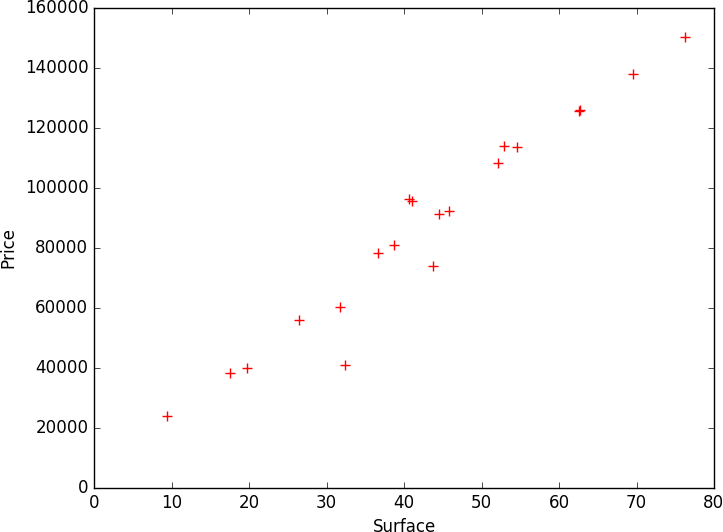
\includegraphics[height=.5\textheight]{./fig/surf_price.png}
\end{figure}
\pause
\column{0.4\textwidth}
\begin{block}{}
Questions asked given the data:
\end{block}
\begin{itemize}[<+->]
\item Is there a relationship between the surface and the price?
\item If so, Can we define this relationship?
\item Can we predict the price of appartement with a given surface?
\item What is the error of this prediction ?
\end{itemize}
\end{columns}
\end{frame}

%%%%%%%%%%%%%%%%%%%%%
\begin{frame}
\frametitle{Vocabulary}
\begin{itemize}
\item<1-> the set $\{(x_1,y_1),\ldots,(x_n,y_n)\}$ is called the \alert{learning dataset},

where:
\begin{itemize}
\item Variables $x_i$ are called the \alert{predictors}
\item Variables $y_i$ are called the \alert{targets}
\end{itemize}

\item<2-> A \alert{model}, or the hypothesis function is denoted $h_\theta(x)$ and is defined as:
$$
y_i = h_\theta(x_i) + e_i
$$
where:
\begin{itemize}
\item $e_i$ the error of the model or the \alert{residual}.
\item $\theta \in \R^p$ is a parameter of the function $h_\theta(x)$.
\end{itemize}
\item<3-> We define a \alert{prediction} $\hat{y}$ to be the output of the model given a particular $x$:
$\hat{y} = h_\theta(x)$.
\end{itemize}
\pause[4]
\begin{alertblock}{}
The prediction of a numerical variable $y$ from a predictor $x$ given a learning dataset is called
a \alert{regression}.
\end{alertblock}

\end{frame}

\begin{frame}
\frametitle{The probabilistic point of view}
$e_i$ is considered as the realization of a random variable $\epsilon_i$.
So $y_i$ (depending on $e_i$) is also a realization of a random variable $Y_i$
with the expression
$$
Y_i = h_\theta(x_i) + \epsilon_i
$$

For the further results, we need to make two strong hypothesis:
\begin{exampleblock}{Hypothesis 1}
$$\forall i, \E[\epsilon_i]=0$$
\end{exampleblock}

\begin{exampleblock}{Hypothesis 2}
$\Var(\epsilon_i)=\sigma^2$ and $\forall i \neq j, \epsilon_i$ and $\epsilon_j$ are independant.
\end{exampleblock}

\begin{alertblock}{Danger !}
Very often, the hypothesis 2 is not verified.
\end{alertblock}

\note{show why hypothesis 2 is hard}

\end{frame}


%%%%%%%%%%%%%%%%%%%%%
\begin{frame}
\frametitle{Choice of the hypothesis}
\begin{block}{}
In linear regression, the function $\h$ is assumed to be linear:
$$
\h = \theta_0 + \theta_1 x
$$

\end{block}
\begin{itemize}
\item Linear regression is often (always) the first model to test
\item Some non-linear models can be handled through linear regression (using a transformation of
the predictor $x$ or the target $y$).
\end{itemize}
\end{frame}

%%%%%%%%%%%%%%%%%%%%%
\begin{frame}
\frametitle{Other examples of dependencies}
\begin{columns}
\column{.5\textwidth}
\vspace{-2em}
\begin{figure}
Positive linear with noise\\
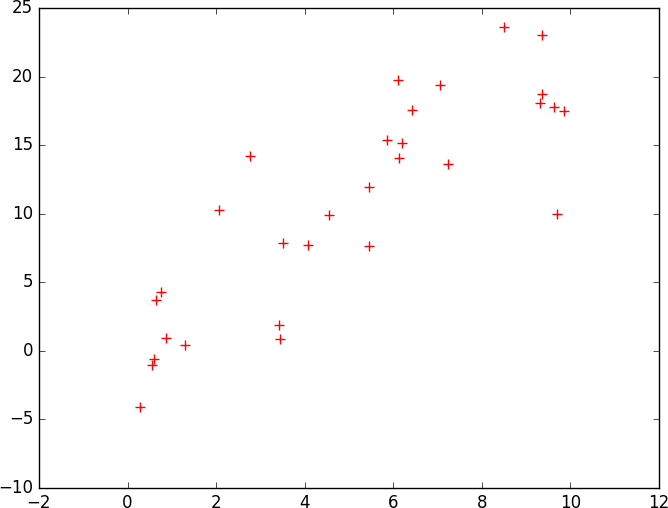
\includegraphics[height=.38\textheight]{./fig/positive.png}
\end{figure}
\vspace{-2em}
\begin{figure}
Negative linear\\
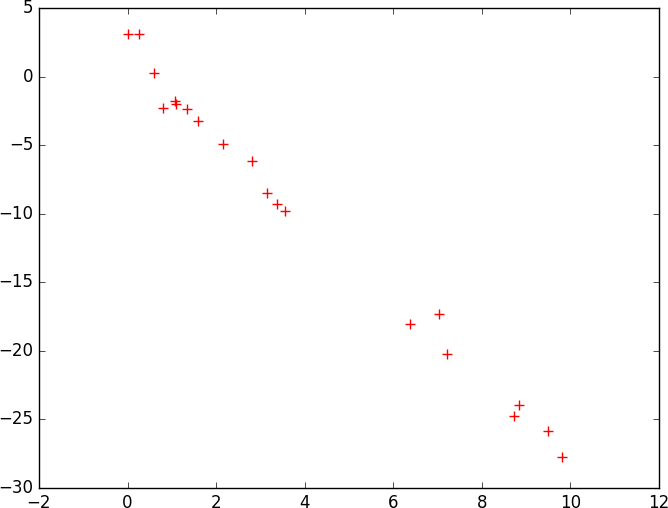
\includegraphics[height=.38\textheight]{./fig/negative.png}
\end{figure}
\column{.5\textwidth}
\vspace{-2em}
\begin{figure}
Non-linear \\
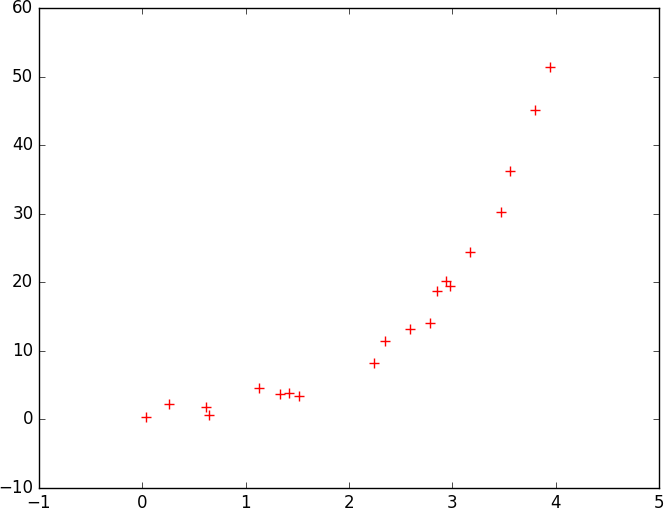
\includegraphics[height=.38\textheight]{./fig/nolinear.png}
\end{figure}
\vspace{-2em}
\begin{figure}
No dependancy\\
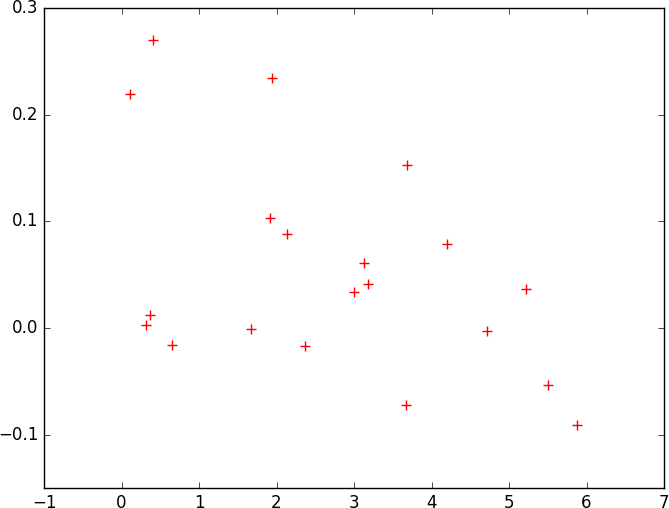
\includegraphics[height=.38\textheight]{./fig/nolink.png}
\end{figure}

\end{columns}
\end{frame}
%%%%%%%%%%%%%%%%%%%%
\begin{frame}
\frametitle{Estimation of the parametre $\theta$}
\begin{itemize}
\item Learning dataset: $\{(x_1,y_1),\ldots,(x_n,y_n)\}$
\item Hypothesis function: $\h = \theta_0 + \theta_1 x$
\end{itemize}
\begin{block}{The principle}
Estimating $\theta=(\theta_0,\theta_1)$ is performed by
minimizing the misfit between targets $y_i$ and 
predictions $\hat{y_i}=h_\theta(x_i)$ for $i \in \{1,\ldots,n\}$.
So $\hat{\theta_0}$ and $\hat{\theta_1}$ are chosen such as:
$$
J(\theta_0,\theta_1) = \sum_{i=1}^n D(h_\theta(x_i),y_i)
$$
is minimum.
\end{block}

\begin{alertblock}{}
What is chosen for the misfit $D$ ?
\end{alertblock}
\end{frame}

%%%%%%%%%%%%%%%%%%%%%
\begin{frame}
\frametitle{The least-mean square}
\begin{block}{The last-mean square function}
$$
D(\hat{y},y)= \frac{1}{2}(\hat{y} - y)^2
$$
\end{block}
We can rewrite $J:$
$$
J(\theta_0,\theta_1) =\frac{1}{2} \sum_{i=1}^n (y_i - \theta_0 - \theta_1 x_1)^2
$$
\begin{alertblock}{Determination of $\hat{\theta}_0$ and $\hat{\theta}_1$}
$$
\hat{\theta}_0 = \overline{y} - \hat{\theta}_1\overline{x}
$$
where $\overline{y}=\frac{1}{n}\sum y_i$ and $\overline{x}=\frac{1}{n}\sum x_i$ are the mean values
and:
$$
\hat{\theta}_1 = \frac {\sum_{i=1}^n (x_i-\overline{x})y_i}
{\sum_{i=1}^n (x_i-\overline{x})^2}
$$
\end{alertblock}
\note{explain the factor 0.5, make the demonstration}
\end{frame}

%%%%%%%%%%%%%%%%%%%%
\begin{frame}
\frametitle{Some remarks}
\begin{itemize}
\item From $\hat{\theta}_0 = \overline{y} - \hat{\theta}_1\overline{x}$, we conclude
that the center of gravity $(\overline{x},\overline{y})$ is on the regression line.
\item We can derive the theoritical property:
$$
\hat{\theta}_0 = \theta_0 + \frac{\sum(x_i - \overline{x})e_i}{\sum(x_i - \overline{x})^2}
$$
\end{itemize}
\end{frame}

%%%%%%%%%%%%%%%%%%%%%%
\begin{frame}
\frametitle{Some probabilistic properties}
\begin{block}{}
$\hat{\theta}_0$ and $\hat{\theta}_1$ are estimators of the parameters $\theta_0$ and
$\theta_1$
\end{block}
\begin{itemize}
\item Estimators are unbiased, $\E[\hat{\beta}_0] = \beta_0$ and $\E[\hat{\beta}_1] = \beta_1$
\item $\Var(\hat{\beta}_0)=\sigma^2\left( \frac{1}{n} + \frac{\overline{x}^2}{\sum(x_i - \overline{x})^2} \right)$
\item $\Var(\hat{\beta}_1)=\frac{\sigma^2}{\sum(x_i - \overline{x})^2)}$
\item with the assumption that $\epsilon_i \sim \mathcal{N}(0,\sigma)$, we can demonstrate that
$\hat{\theta}_0$ and $\hat{\theta}_1$ are maximum likelihood estimators. It means, it maximize:
$p(Y_i=y_i | \theta_0,\theta_1, x_i)$
\end{itemize}

\note{rewrite relation in term of random values}
\end{frame}

%%%%%%%%%%%%%%%%
\begin{frame}
\frametitle{Residuals}
\begin{block}{Estimation of residual}
We estimate the residuals $\epsilon_i$ using the formula:
$$
\hat{\epsilon}_i = y_i - \hat{\theta}_0 - \hat{\theta}_1 x_i =
(y_i - \overline{y}) - \theta_1(x_i - \overline{x})
$$
\end{block}
Note that $ \sum \hat{\epsilon}_i =0 $.

\begin{block}{Estimation (unbiased) of $\sigma$}
$$\hat{\sigma}^2 = \sum \frac{\hat{\epsilon}_i^2}{n-2}$$
\end{block}
\note{make a graphic representation}
\end{frame}
%%%%%%%%%%%%%%%%
\begin{frame}
\frametitle{Prediction}

Making a prediction is to estimate the target $y$ given a new variable $x_{n+1}$
under the assumption that $y$ is following the same model:
$$Y_{n+1} = \theta_0 + \theta_1 x_{n+1} + \epsilon_{n_1}
$$
\begin{block}{Predicted value}
$$\hat{y}_{n+1} = h_\theta(x_{n+1}) = \theta_0 + \theta_1x_{n+1}$$
\end{block}
Property of the prediction error $\hat{\epsilon}_{n+1} = \hat{y}_{n+1} - y_{n+1}$:
\begin{itemize}
\item $\E[\hat{\epsilon}_{n+1} ] = 0$
\item $\Var(\hat{\epsilon}_{n+1} ) = \sigma^2 
\left(  1 + \frac{1}{n} + \frac{(x_{n+1} -\overline{x})^2}{\sum(x_i - \overline{x})^2}\right)$
\end{itemize}

\end{frame}

%%%%%%%%%%%%%%%%%%%%
\begin{frame}
\frametitle{geometric interpretation}

Let's denote $\bm{x}=(x_1,\ldots,x_n)^T$ and 
$\bm{y}=(y_1,\ldots,y_n)^T$
$\bm{x}$ and $\bm{y} \in \R^n$
\begin{block}{Linear regression as a projection}
The linear regression estimate:
$\bm{\hat{y}} = \hat{\theta}_0 + \hat{theta}_1 \bm{x}$,
$\bm{\hat{y}} = \{\hat{y}_1,\ldots,\hat{y}_n \}$ 
is belonging to the subspace $\mathcal{M}(\bm{x})$ of dimension 2 spanned by vectors
$\bm{x}$  and $\bm{1} = (1,\ldots,1)^T$
and is the orthogonal projection of $\bm{y}$ on $\mathcal{M}(\bm{x})$
\end{block}
Note that (by definition) the orthogonal projection minimize the norm $\| \bm{\hat{y}} - \bm{y} \|$
\note{make a draw here}
\end{frame}

%%%%%%%%%%%%%%%%%%%%%

\begin{frame}
\frametitle{Multivariate linear regression}
Example of surface/price + number of rooms + Age of the building + floor
\end{frame}

%%%%%%%%%%%%%%%%%%%%%
\begin{frame}
\frametitle{New hypothesis model}
Say about $X^0=1$
\end{frame}
%%%%%%%%%%%%%%%%%%%%%
\begin{frame}
\frametitle{Finding theta}
Pseudo-invers
\end{frame}

\begin{frame}
\frametitle{Gradient descent method}
\end{frame}


\end{document}